\chapter{$\mathbf{\symBSPsweep}$}
\label{hoofdstuk:bsp-sweep}
In dit hoofdstuk wordt een nieuw soort $\symBSP$ boom besproken: de $\symBSPsweep$ boom.
Eerst wordt het nut van het opsplitsen van bladknopen in kleinere bladknopen wiskundig besproken en aangetoond met behulp van een voorbeeld.
Het algemene idee van de $\symBSPsweep$ boom wordt dan besproken en daarna worden een aantal specifieke versies van de $\symBSPsweep$ ($\symBSPrandom$, $\symBSParbitrary$ en $\symBSPcluster$) besproken.

\section{Probleemstelling}
    Het doel van acceleratiestructuren is om de totale tijd nodig om een scene te renderen, te minimaliseren.
    Deze sectie toont aan dat de totale rendertijd afhankelijk is van het aantal driehoeken in de geïntersecteerde bladknopen.
    In de eerste subsectie wordt wiskundig aangetoond dat het (onder bepaalde aannames) altijd voordelig is om bladknopen met meer dan één driehoek op te splitsen in kleinere bladknopen.
    De tweede subsectie toont een voorbeeld waarbij de $\symKd$ en $\symBSPize$ boom vergeleken worden op basis van de grootte van de bladknopen.
\subsection{Wiskundige basis}
    De rendertijd $\symTime_{\symRender}$ bestaat uit twee grote factoren: de tijd gespendeerd aan het intersecteren met driehoeken (de intersectietijd) en de tijd gespendeerd aan het doorkruisen van de boom (de doorkruistijd).
    De totale intersectietijd $\symTime_{\symIntersection, \symTotal}$ is afhankelijk van het aantal driehoeken $\symNbPrimitives_\symLeaf$ in de geïntersecteerde bladknopen $\symLeaf$ en het aantal keer $\symTraversalL_\symLeaf$ dat elk van deze bladknopen doorkruist wordt.
    De totale doorkruistijd $\symTime_{\symTraversal, \symTotal}$ is afhankelijk van het aantal doorkruisingen $\symTraversalL_{\symInternal}$ van inwendige knopen.
    Formule \ref{eq:rendertijd} beschrijft dit wiskundig met $\symTime_{\symIntersection}$ de tijd nodig voor één straal-driehoekintersectie, $\symTime_{\symTraversal}$ de tijd nodig om één knoop te doorkruisen en $B$ het aantal geïntersecteerde bladknopen.
\begin{equation}
    \label{eq:rendertijd}
   \symTime_{\symRender} \sim
    \symTime_{\symIntersection, \symTotal} + \symTime_{\symTraversal, \symTotal} = \symTime_{\symIntersection} * \sum_{\symLeaf}^\symLeafL \symNbPrimitives_\symLeaf * \symTraversalL_\symLeaf + \symTime_{\symTraversal} * \symTraversalL_{\symInternal}
\end{equation}

Stel dat één kindknoop $\symLeaf_j$ uit de boom wordt opgesplitst in twee kleinere kindknopen $\symLeaf_{j1}$ en $\symLeaf_{j2}$ die elk de helft van de driehoeken krijgen.
Deze opsplitsing is voordelig als aan voorwaarde \ref{eq:vw_splitwinst} voldaan is.
Deze voorwaarde drukt uit dat knoop $\symLeaf_j$ nu een inwendig knoop wordt en dus niet meer zorgt voor een intersectietijd en wel voor een doorkruistijd en dat de nieuwe kindknopen zorgen voor een intersectietijd.
De voorwaarde is equivalent aan voorwaarden \ref{eq:vw_splitwinst_tussen} en \ref{eq:vw_splitwinst_res}.
% B -> 2Bs : nb -> nb/2 * 2 en Db1 + db2 << Db + 1 inwendige knoop, Db keer bekeken
\begin{equation}
    \label{eq:vw_splitwinst}
    \symTime_{\symRender} - \symTime_{\symIntersection} * \symNbPrimitives_{\symLeaf_j} * \symTraversalL_{\symLeaf_j} + \symTime_{\symTraversal} * \symTraversalL_{\symLeaf_j}  + \frac{\symNbPrimitives_{\symLeaf_j}}{2} * (\symTraversalL_{\symLeaf_{j1}} + \symTraversalL_{\symLeaf_{j2}}) * \symTime_{\symIntersection} \leq \symTime_{\symRender}
\end{equation}
\begin{equation}
    \label{eq:vw_splitwinst_tussen}
  \Leftrightarrow \frac{\symNbPrimitives_{\symLeaf_j}}{2} * (\symTraversalL_{\symLeaf_{j1}} + \symTraversalL_{\symLeaf_{j2}}) * \symTime_{\symIntersection} \leq (\symTime_{\symIntersection} * \symNbPrimitives_{\symLeaf_j} - \symTime_{\symTraversal}) * \symTraversalL_{\symLeaf_j}
\end{equation}
%\begin{equation}
%    \frac{\symNbPrimitives_{\symLeaf_j} * \symTime_{\symIntersection}}{(\symTime_{\symIntersection} * \symNbPrimitives_{\symLeaf_j} - \symTime_{\symTraversal})} \leq \frac{2\symTraversalL_{\symLeaf_j}}{(\symTraversalL_{\symLeaf_{j1}} + \symTraversalL_{\symLeaf_{j2}}) }
%\end{equation}
%\begin{equation}
%    \frac{1}{(1 - \frac{\symTime_{\symTraversal}}{\symNbPrimitives_{\symLeaf_j} * \symTime_{\symIntersection}})} \leq \frac{2\symTraversalL_{\symLeaf_j}}{(\symTraversalL_{\symLeaf_{j1}} + \symTraversalL_{\symLeaf_{j2}}) }
%\end{equation}
\begin{equation}
    \label{eq:vw_splitwinst_res}
    \Leftrightarrow \symTraversalL_{\symLeaf_{j1}} + \symTraversalL_{\symLeaf_{j2}} \leq
    2\symTraversalL_{\symLeaf_j} * (1 - \frac{\symTime_{\symTraversal}}{\symNbPrimitives_{\symLeaf_j} * \symTime_{\symIntersection}})
\end{equation}

De som in het linkerlid van voorwaarde \ref{eq:vw_splitwinst_res} is minstens gelijk aan $\symTraversalL_{\symLeaf_{j}}$ aangezien elke doorkruising van $\symLeaf_j$ voor minstens één doorkruising door een kindknoop zorgt.
Analoog kan worden ingezien dat de maximale waarde voor deze som gelijk is aan $2\symTraversalL_{\symLeaf_{j}}$ aangezien elke doorkruising van $\symLeaf_j$ voor maximaal twee doorkruisingen door een kindknoop kan zorgen. Hieruit volgt ongelijkheid \ref{eq:vw_doorkruisingen}.

\begin{equation}
    \label{eq:vw_doorkruisingen}
    \symTraversalL_{\symLeaf_{j}} \leq \symTraversalL_{\symLeaf_{j1}} + \symTraversalL_{\symLeaf_{j2}} \leq 2\symTraversalL_{\symLeaf_{j}}
\end{equation}

In het algemeen geval geldt dat $\symTraversalL_{\symLeaf_{j1}} + \symTraversalL_{\symLeaf_{j2}} = (2 * (1-\beta) + \beta) \symTraversalL_{\symLeaf_{j}}$ waarbij $\beta$ het procentueel aantal doorkruisingen is dat door slechts één van de twee kindknopen gaat.
In dit geval leidt voorwaarde \ref{eq:vw_splitwinst_res} tot voorwaarde \ref{eq:vw_splitwinst_general}.
\begin{equation}
    \label{eq:vw_splitwinst_general}
    (2 * (1-\beta) + \beta) \symTraversalL_{\symLeaf_{j}} \leq
    2\symTraversalL_{\symLeaf_j} - \frac{2\symTraversalL_{\symLeaf_j}\symTime_{\symTraversal}}{\symNbPrimitives_{\symLeaf_j} \symTime_{\symIntersection}}
    \Leftrightarrow
    2 - \beta \leq 2 - \frac{2\symTime_{\symTraversal}}{\symNbPrimitives_{\symLeaf_j} \symTime_{\symIntersection}}
    \Leftrightarrow
    \symTime_{\symTraversal} \leq \frac{\beta \symNbPrimitives_{\symLeaf_j} }{2}\symTime_{\symIntersection}
\end{equation}

In het ideale geval ($\beta = 1$) leidt voorwaarde \ref{eq:vw_splitwinst_general} tot $\symTime_{\symTraversal} \leq \frac{\symNbPrimitives_{\symLeaf_j}}{2}\symTime_{\symIntersection}$.
Het opsplitsen van een knoop met twee driehoeken, kan hierdoor pas voordelig zijn als de doorkruistijd kleiner is dan de intersectietijd.
Aangezien de doorkruistijd in de realiteit beduidend kleiner is dan de intersectietijd, is het in dit ideale geval altijd voordelig om een kindknoop op te splitsen, ongeacht het aantal driehoeken in de knoop.
In het slechtste geval ($\beta = 0$) kan aan voorwaarde \ref{eq:vw_splitwinst_general} enkel voldaan zijn als de doorkruistijd gelijk is aan nul. Dit is onmogelijk waardoor opsplitsen nooit voordelig kan zijn in dit geval. \\

Het is moeilijk om de waarde van $\beta$ te voorspellen, deze is namelijk afhankelijk van de exacte stralen die tijdens het renderen gevolgd worden, de specifieke driehoeken in de knoop en het splitsingsvlak. 
Voorwaarde \ref{eq:vw_splitwinst_general} toont dat de kans dat splitsen voordelig is, lineair stijgt met $\symNbPrimitives_{\symLeaf_j}$. 
De voorwaarde toont ook dat het splitsen van een knoop met twee driehoeken, voordelig is wanneer de doorkruistijd $\beta$ keer kleiner is dan de intersectietijd. 
Intuïtief lijkt het logisch dat hier in het algemeen aan voldaan is. 
Hieruit kan worden afgeleid dat het altijd beter is om bladknopen met meer dan één driehoek op te splitsen in twee kleinere bladknopen.\\

\subsection{Voorbeeld}
  \begin{figure}
    \begin{subfigure}{0.4\textwidth}
        \centering
        \begin{subfigure}{\textwidth}
            \centering
            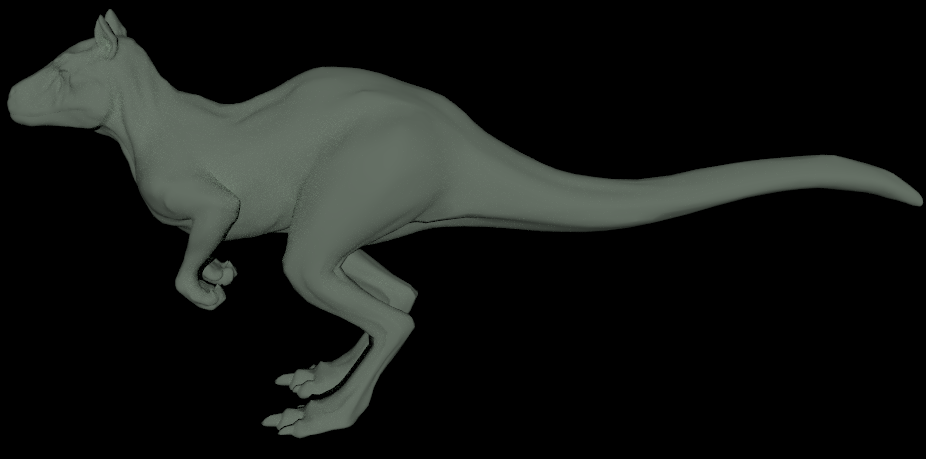
\includegraphics[width=1\linewidth]{img/killeroo}
            \caption{Killeroo scene}
            \label{fig:killeroo}    
        \end{subfigure}
        \begin{subfigure}{\textwidth}
            \centering
            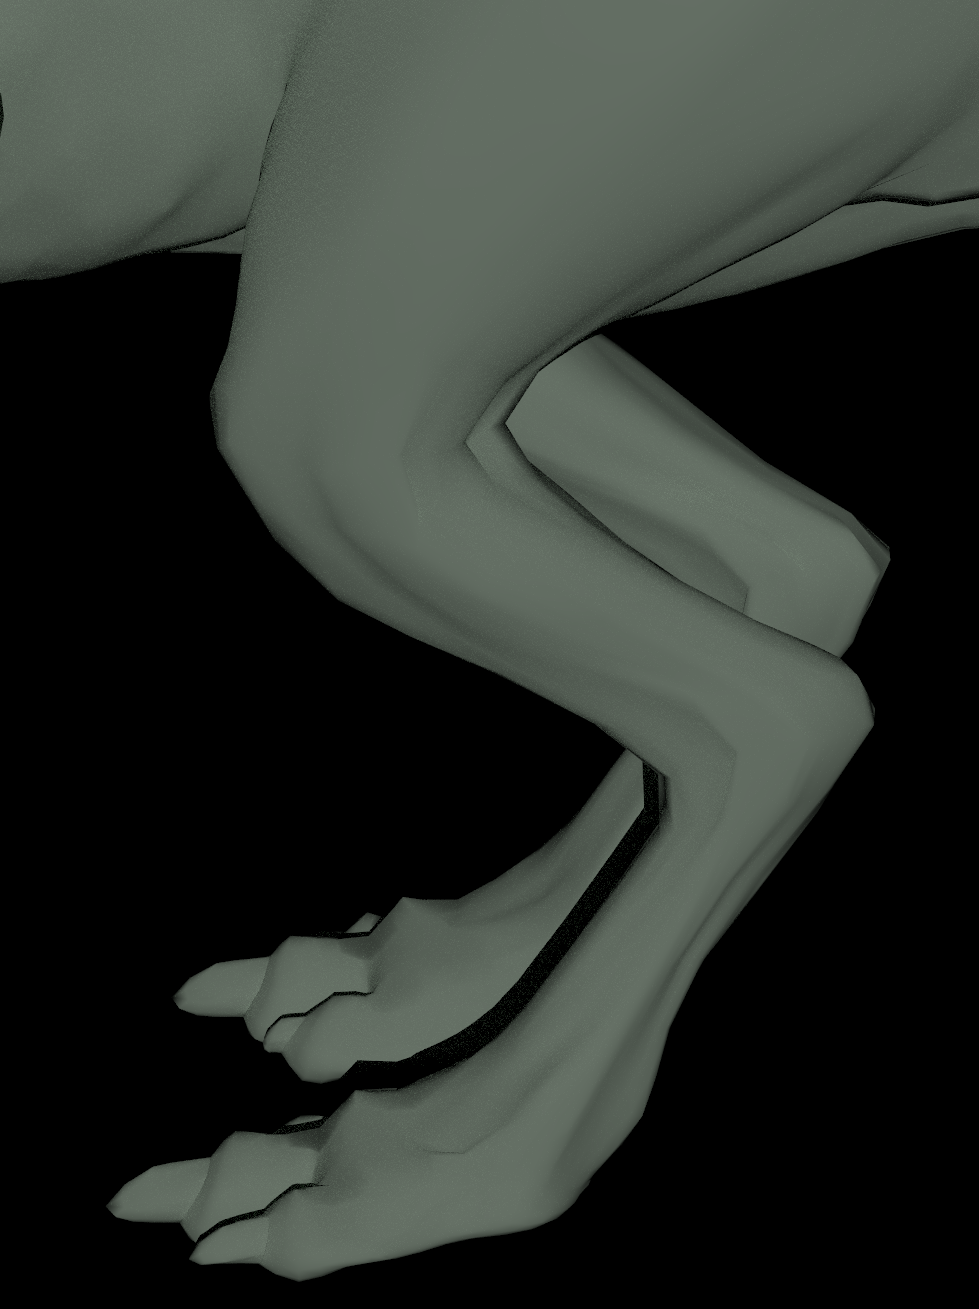
\includegraphics[width=0.5\linewidth]{img/killerooFeet}
            \caption{Killeroo Been scene}
            \label{fig:killeroo-been}    
        \end{subfigure}
    \end{subfigure}
    \begin{subfigure}{0.5\textwidth}
        \centering
    \begin{tikzpicture}[scale=0.6]
        \begin{axis}[
          axis lines = left,
          ylabel = \small Cumulatieve bijdrage aan totaal aantal straal-driehoekintersecties,
          xlabel = \small Aantal driehoeken in bladknoop,
          ymin=1000000, ymax=180000000,
          width=1.6\textwidth,
          height=2\textwidth,
          cycle multi list={%
            color list\nextlist
            [2 of]mark list
          },
          title = \small,
          legend pos=north west,
      ]
        \addplot table [x=V1, y=KillerooKdTotal, col sep=comma] {data/killeroo_feet_kd_bsp.csv};
        \addlegendentry{$\symKd$ Killeroo}
        \addplot table [x=V1, y=FeetKdTotal, col sep=comma] {data/killeroo_feet_kd_bsp.csv};
        \addlegendentry{$\symKd$ Killeroo Been}
    
        \addplot table [x=V1, y=KillerooBSPTotal, col sep=comma] {data/killeroo_feet_kd_bsp.csv};
        \addlegendentry{$\symBSPizefastkd$ Killeroo}
        \addplot table [x=V1, y=FeetBSPTotal, col sep=comma] {data/killeroo_feet_kd_bsp.csv};
        \addlegendentry{$\symBSPizefastkd$ Killeroo Been}
        
          \end{axis}
        \end{tikzpicture}
        \caption{Cumulatief aantal straal-driehoekintersecties}
        \label{fig:voorbeeld-cumul}
    \end{subfigure}
    \label{fig:voorbeeld-bladknopen}
    \caption[Invloed grootte bladknopen op het aantal straal-driehoekintersecties]{Invloed grootte bladknopen op het aantal straal-driehoekintersecties - \small (a) toont de Killeroo scene, (b) toont de scene waarbij ingezoomd is op de benen van de Killeroo, (c) toont het totaal aantal intersecties als een cumulatieve som over het aantal driehoeken in de bladknoop. Dit betekent dat de waarde bij x overeenkomt met de som van het aantal intersecties in bladknopen met x of minder driehoeken.}
\end{figure}
Figuur \ref{fig:killeroo} toont de Killeroo scene die als voorbeeld scene dient bij de pbrt \cite{pbrt} \textit{ray tracer}.
Voor deze scene zijn de $\symKd$ boom en de $\symBSPizefastkd$ boom aan elkaar gewaagd.
De $\symBSPizefastkd$ boom neemt de bovenhand als er wordt ingezoomd op de benen (figuur \ref{fig:killeroo-been}) van de Killeroo, waar de $\symKd$ boom veel bladknopen met meerdere driehoeken bevat.
Figuur \ref{fig:voorbeeld-cumul} toont het cumulatief aantal intersecties per groep van bladknopen met hetzelfde aantal driehoeken.
Voor de gewone Killeroo scene, heeft de $\symKd$ boom slechts een beperkt aantal extra intersecties nodig.
Bij de ingezoomde scene, komt een groot deel van de intersecties van de $\symKd$ boom door intersecties met bladknopen met een groot aantal driehoeken.
Dit toont aan dat algemene $\symBSP$ bomen nuttig kunnen zijn omdat ze in principe alle niet-intersecterende driehoeken van elkaar kunnen scheiden en er dus minder regio's zijn met veel grote bladknopen.
Het aantal knoopdoorkruisingen bij de $\symBSPizefastkd$ boom is zelfs lager dan bij de $\symKd$ boom voor beide scenes.
Dit komt omdat de algemene $\symBSP$ bomen nauwer aansluiten aan het object waardoor minder stralen de knopen raken.\\

Figuur \ref{fig:killeroo-heatmaps} toont \textit{false color} afbeeldingen van het aantal zichtstraalintersecties van de Killeroo en Killeroo Been scene voor zowel de $\symKd$ boom als de $\symBSPizefastkd$ boom. 
Voor de Killeroo scene zijn de \textit{false color} afbeeldingen van beide bomen zeer gelijkaardig, maar aan de benen heeft de $\symKd$ boom duidelijk meer intersecties nodig.
Dit wordt bevestigd door de \textit{false color} afbeeldingen van de Killeroo Been scene waarop duidelijk zichtbaar is dat de $\symBSPizefastkd$ boom zich beter kan aanpassen aan complexe geometrie.
Het is ook zichtbaar dat de $\symBSPizefastkd$ boom nauwer aansluit aan de scene dan de $\symKd$ boom.
Merk op dat, zoals besproken in het vorige hoofdstuk, de $\symBSPizefastkd$ boom nog niet alle vrijheiden van een algemene $\symBSP$ boom gebruikt.\\

\begin{figure}
    \begin{subfigure}{0.5\textwidth}
        \centering
        \begin{subfigure}{\textwidth}
            \centering
            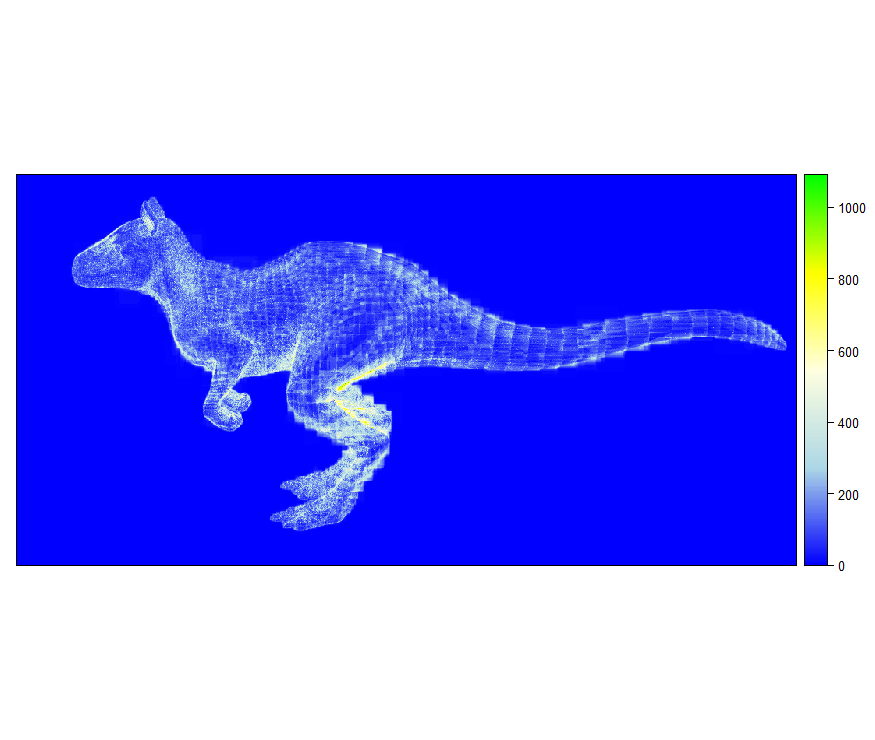
\includegraphics[width=1\linewidth]{img/killeroo-kd-heatmap}
            \caption{Killeroo $\symKd$}
            \label{fig:killeroo-kd-heatmap}    
        \end{subfigure}
        \begin{subfigure}{\textwidth}
            \centering
            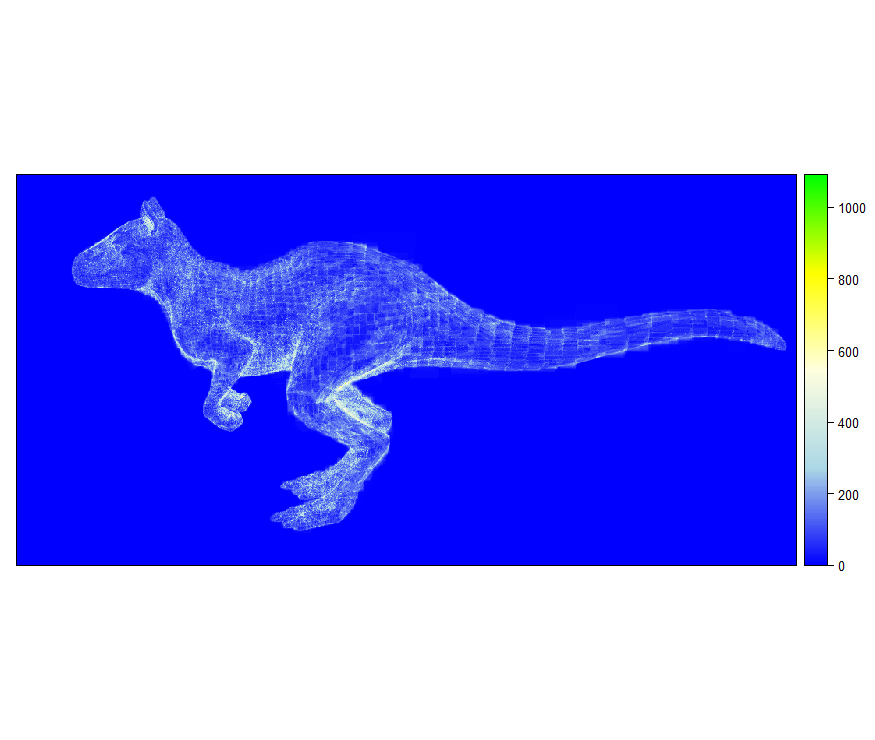
\includegraphics[width=1\linewidth]{img/killeroo-bspize-heatmap}
            \caption{Killeroo $\symBSPizefastkd$}
            \label{fig:killeroo-bspize-heatmap}    
        \end{subfigure}
    \end{subfigure}
    \begin{subfigure}{0.5\textwidth}
        \centering
        \begin{subfigure}{\textwidth}
            \centering
            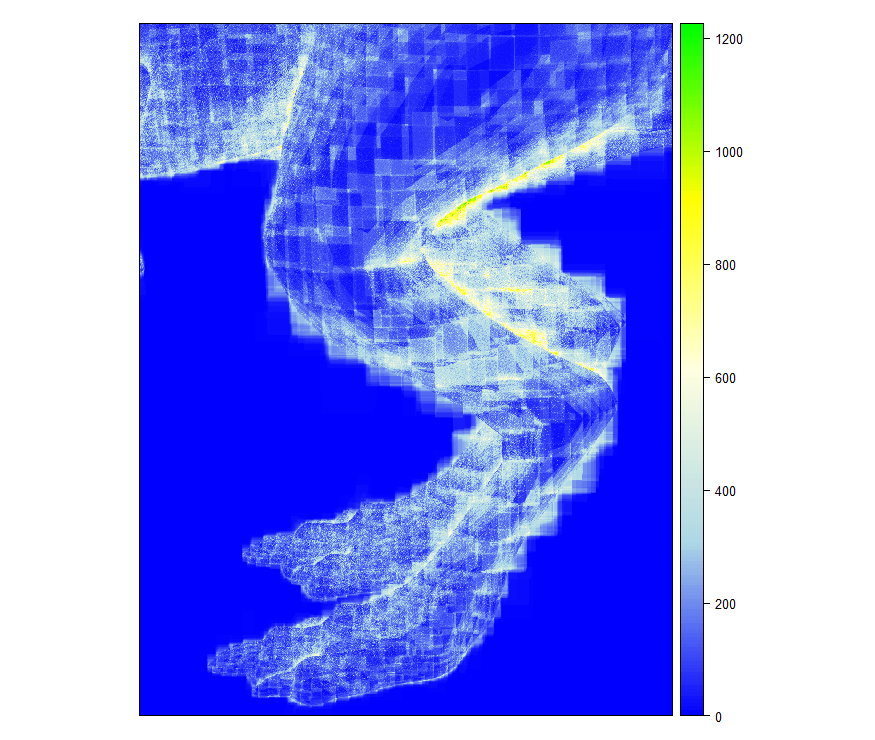
\includegraphics[width=1\linewidth]{img/killeroo-feet-kd-heatmap}
            \caption{Killeroo Been $\symKd$}
            \label{fig:killeroo-been-kd-heatmap}    
        \end{subfigure}
        \begin{subfigure}{\textwidth}
            \centering
            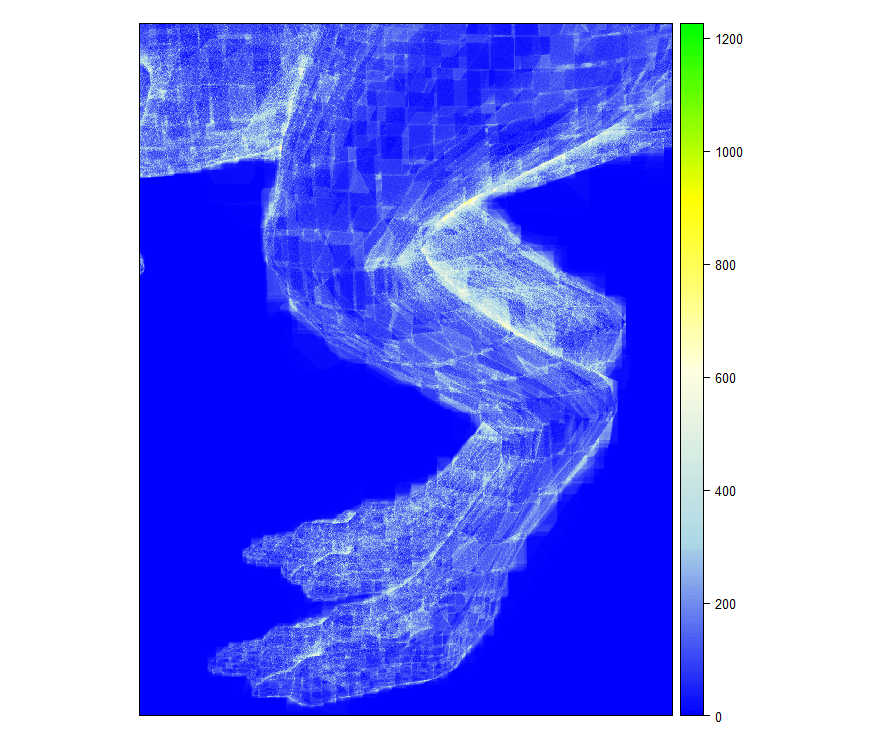
\includegraphics[width=1\linewidth]{img/killeroo-feet-bspize-heatmap}
            \caption{Killeroo Been $\symBSPizefastkd$}
            \label{fig:killeroo-been-bspize-heatmap}    
        \end{subfigure}
    \end{subfigure}
    \caption[\textit{False color} afbeeldingen van de Killeroo en Killeroo Been scene]{\textit{False color} afbeeldingen van de Killeroo en Killeroo Been scene - \small Deze afbeeldingen tonen dat de $\symKd$ boom slecht presteert bij sommige delen van een scene, in dit geval de benen van de Killeroo. Bij de $\symBSPizefastkd$ boom is dit fenomeen veel minder uitgesproken en het valt ook op dat de $\symBSPizefastkd$ boom nauwer aansluit aan de scene.}
    \label{fig:killeroo-heatmaps}
\end{figure}

De volgende secties bespreken nieuwe $\symBSP$ bomen die gebruik maken van de vrijheid om op elk niveau van de boom andere splitsingsvlakken te gebruiken. Op die manier kunnen ze meer bladknopen opsplitsen in kleinere bladknopen en nog nauwer aansluiten aan de scene.\\



\section{Concept}
    De $\symBSPsweep$ boom is een algemene $\symBSP$ boom waarbij in elke knoop k richtingen bepaald worden en alle $2n$ splitsingsvlakken langs elk van deze richtingen bekeken worden door te sweepen.
    Deze k richtingen kunnen verschillend zijn voor elke knoop en kunnen gekozen worden afhankelijk van de lokale geometrie.
    De $\symRBSP$ boom is een $\symBSPsweep$ boom waarbij de gekozen richtingen in elke knoop hetzelfde zijn.
    De $\symBSPsweep$ boom heeft drie belangrijke ontwerpbeslissingen.
    De belangrijkste ontwerpbeslissing bij de $\symBSPsweep$ boom is de methode die gebruikt wordt om de k richtingen te bepalen.
    Een tweede belangrijke ontwerpbeslissing is de waarde van k.
    De derde belangrijke ontwerpbeslissing sluit aan bij de eerste en gaat over het al dan niet gebruiken van de $\symKd$ richtingen als de eerste drie van de k richtingen.
    \\


    %Kd-richtingen + aantal richtingen of puur die richtingen
    %Snelle traversal voor kd-richtingen
\section{Gebaseerd op random richtingen}
De simpelste $\symBSPsweep$ boom, de $\symBSPrandom$ boom, bepaalt in elke knoop k random richtingen onafhankelijk van de geometrie.
De richtingen worden uniform op de hemisfeer gegenereerd.
Het idee achter deze boom is dat het nuttiger kan zijn om te proberen om driehoeken te splitsen via veel verschillende  (mogelijks slechte) vlakken, dan om ze steeds met dezelfde vlakken te proberen te splitsen.
Als de driehoeken in de scene uniform verdeeld zijn, dan is de kans dat twee driehoeken volgens een willekeurige richting gesplitst kunnen worden, even groot als de kans dat ze door een $\symKd$ richting gesplitst kunnen worden.\\

Als de $\symBSPrandom$ boom perfect gebalanceerd is, worden in elk niveau $2kn$ verschillende splitsingsvlakken bekeken.
Deze splitsingsvlakken zijn verschillend op elk niveau, zodat in totaal $2knlog(n)$ verschillende splitsingsvlakken bekeken worden.
Figuur \ref{fig:splitsingsvlakken-bsprandom} toont dit visueel.
De $\symBSPrandom$ boom probeert elke driehoek via gemiddeld $2klog(n)$ ($\symO(log(n))$) vlakken te splitsen van de andere driehoeken, in tegenstelling tot de bestaande bomen die dit maximaal met $\symO(1)$ vlakken proberen.\\

\begin{figure}
    \centering

   \resizebox{0.4\textwidth}{!}{%
   \centering
    \begin{tikzpicture}
   \Tree
   [ .\node[fill=green]{$2kn$};    
       [.\node[fill=nodeblue1]{$2k\frac{n}{2}$};
           [.\node(n3l)[fill=nodered1, text=white]{$2k\frac{n}{4}$};]
           [.\node[fill=nodered2, text=white]{$2k\frac{n}{4}$};]
       ]
       [.\node[fill=nodeblue2, text=white]{$2k\frac{n}{2}$};
           [.\node[fill=nodered3, text=white]{$2k\frac{n}{4}$};]
           [.\node(n3r)[fill=nodered4, text=white]{$2k\frac{n}{4}$};]
       ]
   ]
   \node at (3,0.5) {$\#$};
   \node at (4,0.5) {$\# \neq$};
   \node at (3,0) {$2kn$};
   \node at (3,-1.5) {$2kn$};
   \node at (3,-3) {$2kn$};
   \node at (4,0) {$2kn$};
   \node at (4,-1.5) {$4kn$};
   \node at (4,-3) {$6kn$};
   \end{tikzpicture}
   }
   \caption[Splitsingsvlakken $\symBSPrandom$]%
    {Splitsingsvlakken $\symBSPrandom$ - \small Per niveau het aantal ($\#$) splitsingsvlakken en het totaal aantal verschillende ($\# \neq$) splitsingsvlakken gebruikt in bovenliggende niveaus bij de $\symBSPrandom$ boom.} %TODO: meer uitleg
    \label{fig:splitsingsvlakken-bsprandom}
\end{figure}

\begin{figure}
        \resizebox{\textwidth}{!}{%
        \centering
         \begin{tikzpicture}
            \usetikzlibrary{arrows}
            \usetikzlibrary{shapes}
\tikzstyle{every tree node}=[draw, ellipse, align=center]
        \Tree
        [ .\node[shading = axis, left color=green, right color=nodeyellow1,shading angle=135]{$2(k-3)n + 6n$};    
            [.\node[shading = axis, left color=nodeblue1, right color=nodeyellow1, shading angle=135]{$2(k-3)\frac{n}{2} + 6\frac{n}{2}$};
                [.\node(n3l)[shading = axis, left color=nodered1, right color=nodeyellow1, shading angle=135]{$2(k-3)\frac{n}{4} + 6\frac{n}{4}$};]
                [.\node[shading = axis, left color=nodered2, right color=nodeyellow1, shading angle=135]{$2(k-3)\frac{n}{4} + 6\frac{n}{4}$};]
            ]
            [.\node[shading = axis, left color=nodeblue2, right color=nodeyellow1, shading angle=135, text=white]{$2(k-3)\frac{n}{2} + 6\frac{n}{2}$};
                [.\node[shading = axis, left color=nodered3, right color=nodeyellow1, shading angle=135]{$2(k-3)\frac{n}{4} + 6\frac{n}{4}$};]
                [.\node(n3r)[shading = axis, left color=nodered4, right color=nodeyellow1, shading angle=135]{$2(k-3)\frac{n}{4} + 6\frac{n}{4}$};]
            ]
        ]
        \node at (10,0.5) {$\#$};
        \node at (13,0.5) {$\# \neq$};
        \node at (10,0) {$2(k-3)n + 6n$};
        \node at (10,-1.5) {$2(k-3)n + 6n$};
        \node at (10,-3) {$2(k-3)n + 6n$};
        \node at (13,0) {$2(k-3)n + 6n$};
        \node at (13,-1.5) {$4(k-3)n + 6n$};
        \node at (13,-3) {$6(k-3)n + 6n$};
        \end{tikzpicture}
        }
    \caption[Splitsingsvlakken $\symBSPrandomsomekd$]%
    {Splitsingsvlakken $\symBSPrandomsomekd$ - \small Per niveau het aantal ($\#$) splitsingsvlakken en het totaal aantal verschillende ($\# \neq$) splitsingsvlakken gebruikt in bovenliggende niveaus bij de $\symBSPrandomsomekd$ boom.} %TODO: meer uitleg
    \label{fig:splitsingsvlakken-bsprandomsomekd}
\end{figure}

De $\symKd$ richtingen zijn in praktische scenes vaak beter dan willekeurige richtingen omdat ze loodrecht op elkaar staan waardoor ze de hemisfeer goed bedekken en omdat scenes die door de mens gemaakt worden, vaak asgealigneerde delen bevatten.
Dit geeft aanleiding tot een boom die als eerste drie richtingen steeds de $\symKd$ richtingen kiest en enkel de overige $k - 3$ richtingen random genereert: de $\symBSPrandomkd$ boom. Een extra voordeel is dat de snellere $\symKd$ knoopdoorkruising gebruikt kan worden. Een $\symBSPrandom$ boom die altijd de $\symKd$ richtingen gebruikt en de doorkruising van $\symKd$ knopen optimaliseert, wordt aangeduid als $\symBSPrandomfastkd$. 
Als de $\symBSPrandomsomekd$ boom perfect gebalanceerd is, worden in elk niveau $2kn$ splitsingsvlakken bekeken.
Van deze $2kn$ zijn er $6n$ die hergebruikt worden, de vlakken volgens de $\symKd$ richtingen.
Dit zorgt voor $2(k-3)n$ verschillende splitsingsvlakken per niveau, zodat in totaal $2(k-3)nlog(n) + 6n$ verschillende splitsingsvlakken bekeken worden.
Figuur \ref{fig:splitsingsvlakken-bsprandomsomekd} toont dit visueel.
De $\symBSPrandomsomekd$ boom probeert elke driehoek via gemiddeld $\symO(log(n))$ vlakken te splitsen van de andere driehoeken, net als  de $\symBSPrandom$ boom.\\

\section{Gebaseerd op normalen}
    De kracht van de $\symBSPsweep$ boom ligt in het feit dat er gebruik gemaakt kan worden van de lokale geometrie om de splitsingsrichtingen te bepalen.
    De normalen van de driehoeken in een knoop bevatten informatie over de oriëntatie van de driehoeken.
    De autopartitievlakken van \authorIze{} maken ook gebruik van de normalen, maar de normaal van een driehoek wordt enkel voor die driehoek zelf gebruikt.
    
\subsection{Willekeurige normaal}
    De $\symBSParbitrary$ boom is een $\symBSPsweep$ boom waarbij in elke knoop de normalen van k willekeurige driehoeken gekozen worden als splitsingsrichtingenen.
    Als er k of minder driehoeken in de knoop zitten, worden alle normalen als splitsingsrichtingen genomen.
    In het algemeen zijn er n driehoeken met n verschillende normalen waardoor er in totaal $2n^2$ mogelijke splitsingsvlakken zijn.
    Figuur \ref{fig:splitsingsvlakken-bsparbitrary-top} toont het aantal splitsingsvlakken gebruikt per knoop in de bovenste niveaus van de boom.
    Deze figuur is identiek aan de figuur voor de $\symBSPrandom$ boom. \\

    Voor de onderste $log(k)$ niveaus waarop gesplitst wordt - dit zijn de onderste $log(k) + 1$ niveaus behalve het onderste niveau -  is er echter een verschil
    Dit verschil volgt uit het feit dat er in die niveaus k of minder driehoeken in elke knoop zitten.
    In deze onderste $log(k)$ niveaus worden er in elke knoop $2n_m^2$ splitsingsvlakken bekeken, met $n_m <= k$.
    Een knoop op het $m^{de}$ laagste niveau van deze $log(k)$ onderste niveaus bevat $n_m = \frac{n}{2^{log(n) - m}}$ driehoeken waardoor er $2n_m^2 = 2 * (\frac{n}{2^{log(n) - m}})^2 = 2*(2^m)^2 = 2*4^m$ splitsingen gebeuren in deze knoop.
    Formule \ref{eq:bsparbitrary-logkjonderste} toont dat het totaal aantal splitsingsvlakken bekeken op het ${log(k) - j}^{de}$ onderste niveau gelijk is aan $\frac{2kn}{2^j}$. Dit aantal is berekend als het aantal splitsingsvlakken per knoop ($2*4^{log(k) - j}$) vermenigvuldigd met het aantal knopen ($2^{log(n)-log(k)+j}$) op het niveau.
    \begin{equation}
        \label{eq:bsparbitrary-logkjonderste}
    2*4^{log(k) - j} * 2^{log(n)-log(k)+j} = 2 * 2^{log(k) + log(n) - j} = \frac{2 * 2^{log(kn)}}{2^j} =\frac{2kn}{2^j}
    \end{equation}
    In de bovenste $log(n) - log(k) = log(\frac{n}{k})$ niveaus worden $2log(\frac{n}{k})kn$ verschillende splitsingsvlakken bekeken.
    Het niveau eronder gebruikt nog $kn$ nieuwe splitsingsvlakken.
    Dit kan worden ingezien als volgt: de knopen op het niveau erboven bevatten $2k$ driehoeken en in die knoop worden $k$ normalen gekozen, de twee kindknopen van elk van die knopen gebruiken elk k verschillende richtingen en gebruiken dus de volledige $2k$ richtingen waaruit de ouderknoop kon kiezen. Dit betekent dat ze $k$ nieuwe richtingen gebruiken, elk voor de helft van het aantal driehoeken: $2 * k\frac{n}{2} = kn$.
    In totaal worden er $2(log(\frac{n}{k}) + \frac{1}{2})kn$ verschillende splitsingsvlakken worden gebruikt.
    Figuur \ref{fig:splitsingsvlakken-bsparbitrary-bottom} toont dit visueel.
    Als de boom perfect gebalanceerd is, probeert de $\symBSParbitrary$ boom elke driehoek via gemiddeld $2klog(\frac{n}{k} + \frac{1}{2})$ ($\symO(log(n))$) vlakken te splitsen van de andere driehoeken. Dit aantal is minder dan bij de $\symBSPrandom$ boom, die ook in de lagere niveaus steeds k splitsingsrichtingenen genereert.\\

    Net als bij de $\symBSPrandom$ boom kan een versie van de $\symBSParbitrary$ boom gemaakt worden die als eerste drie richtingen steeds de $\symKd$ richtingen kiest en enkel voor de overige $k - 3$ richtingen willekeurige normalen selecteert: de $\symBSParbitrarykd$ boom. Een $\symBSParbitrary$ boom die altijd de $\symKd$ richtingen gebruikt en de doorkruising van $\symKd$ knopen optimaliseert, wordt aangeduid als $\symBSParbitraryfastkd$. Als de $\symBSParbitrarysomekd$ boom perfect gebalanceerd is, worden in totaal $2(log(\frac{n}{k-3}) + \frac{1}{2})(k-3)n + 6n$ verschillende splitsingsvlakken bekeken. De analyse hiervoor is analoog aan de analyse voor $\symBSPrandomsomekd$.

    %TODO: subfig a en b, a zelfde als bsprandom, b = laatste log(k) niveaus -> allemaal dezelfde
    %TODO: kd verbetering -> zelfde formule maar k-3 en + 6n


\begin{figure}
    \centering
    \begin{subfigure}[t]{0.34\textwidth}

   \resizebox{\textwidth}{!}{%
   \centering
    \begin{tikzpicture}
   \Tree
   [ .\node[fill=green]{$2kn$};    
       [.\node[fill=nodeblue1]{$2k\frac{n}{2}$};
           [.\node(n3l)[fill=nodered1, text=white]{$2k\frac{n}{4}$};]
           [.\node[fill=nodered2, text=white]{$2k\frac{n}{4}$};]
       ]
       [.\node[fill=nodeblue2, text=white]{$2k\frac{n}{2}$};
           [.\node[fill=nodered3, text=white]{$2k\frac{n}{4}$};]
           [.\node(n3r)[fill=nodered4, text=white]{$2k\frac{n}{4}$};]
       ]
   ]
   \node at (3,0.5) {$\#$};
   \node at (4,0.5) {$\# \neq$};
   \node at (3,0) {$2kn$};
   \node at (3,-1.5) {$2kn$};
   \node at (3,-3) {$2kn$};
   \node at (4,0) {$2kn$};
   \node at (4,-1.5) {$4kn$};
   \node at (4,-3) {$6kn$};
   \end{tikzpicture}
   }
   \caption{Bovenste drie niveaus}
   \label{fig:splitsingsvlakken-bsparbitrary-top}
\end{subfigure}
\begin{subfigure}[t]{0.64\textwidth}

    \resizebox{\textwidth}{!}{%
    \centering
     \begin{tikzpicture}
        \usetikzlibrary{arrows}
        \usetikzlibrary{shapes}
\tikzstyle{every tree node}=[draw, ellipse, align=center]
    \Tree
    [ .\node[shading = axis, left color=nodeblue1, right color=nodered2,shading angle=90, text=white]{$2*4^{log(k)}$};    
        [.\node[shading = axis, left color=nodeblue1, right color=nodeblue2,shading angle=90, text=white]{$2*4^{log(k) - 1}$};
            [.\node(n3l)[fill=nodeblue1, text=black]{$2*4^{1}$};]
            [.\node[fill=nodeblue2, text=white]{$2*4^{1}$};]
        ]
        [.\node[shading = axis, left color=nodered1, right color=nodered2,shading angle=90, text=white]{$2*4^{log(k) - 1}$};
            [.\node[fill=nodered1, text=white]{$2*4^{1}$};]
            [.\node(n3r)[fill=nodered2, text=white]{$2*4^{1}$};]
        ]
    ]
    \node at (5,0.5) {$\#$};
    \node at (8,0.5) {$\# \neq$};
    \node at (5,0) {$2kn$};
    \node at (5,-1.5) {$kn$};
    \node at (5,-3) {$\frac{kn}{2}$};
    \node at (8,0) {$2(log(\frac{n}{k}) + \frac{1}{2})kn$};
    \node at (8,-1.5) {$2(log(\frac{n}{k}) + \frac{1}{2})kn$};
    \node at (8,-3) {$2(log(\frac{n}{k}) + \frac{1}{2})kn$};
    \end{tikzpicture}
    }
    \caption{Onderste $log(k)$ niveaus}
    \label{fig:splitsingsvlakken-bsparbitrary-bottom}
 \end{subfigure}
   \caption[Splitsingsvlakken $\symBSParbitrary$ en $\symBSPcluster$]%
    {Splitsingsvlakken $\symBSParbitrary$ en $\symBSPcluster$ - \small Per niveau het aantal ($\#$) splitsingsvlakken en het totaal aantal verschillende ($\# \neq$) splitsingsvlakken gebruikt in bovenliggende niveaus bij de $\symBSParbitrary$ en $\symBSPcluster$ bomen.}
\end{figure}

    

    %Extra richtingen door random normalen te kiezen
    %Autopartitie van Ize maar gesweeped
    %Waarom zou dit werken ? : ...
    
\subsection{Geclusterde normalen}
    Bovenstaande $\symBSPsweep$ bomen bevatten een grote niet-deterministische factor.
    De $\symBSPcluster$ boom gebruikt het K-means clustering algoritme om deterministischere richtingen te bepalen.
    Kim et al \cite{kim2002compression} gebruikten een K-means clustering van de normalen om de bestanden van 3D modellen te comprimeren.
    Bij de $\symBSPcluster$ boom worden de normalen van de driehoeken in een knoop geclusterd in k clusters en de centra van deze clusters worden gebruikt als richtingen voor de $\symBSPsweep$ boom.
    Als er k of minder driehoeken in de knoop zitten, worden, net als bij de $\symBSParbitrary$ boom, alle normalen als splitsingsrichting genomen.
    In tegenstelling tot de $\symBSParbitrary$ is het voor de $\symBSPcluster$ moeilijker om het totaal aantal mogelijke splitsingsvlakken te bepalen.
    In het algemeen kan elke clustering verschillende richtingen geven waardoor er oneindig veel mogelijke splitsingsrichtingen mogelijk zijn.
    De $\symBSPcluster$ boom is zeer gelijkaardig aan de $\symBSParbitrary$ boom waardoor het totaal aantal verschillende splitsingsvlakken die gebruikt worden, gelijk is. Analoog bestaan ook de $\symBSPclusterkd$ en $\symBSPclusterfastkd$ bomen.


\section{Samenvatting}
Tabel \ref{tab:boom-vergelijking-sweep} vergelijkt de hierboven besproken $\symBSPsweep$ bomen.
Alle drie bomen zijn algemene $\symBSP$ bomen die een convex veelvlak hebben als omhullend volume.
De $\symBSPsweep$ bomen zijn ontworpen om sweeping te ondersteunen en zo efficiënt, zonder hulpstructuren, de $SAH$ kosten te kunnen berekenen.
De $\symBSPrandom$ boom is onafhankelijk van de lokale geometrie, de twee andere bomen bepalen hun splitsingsvlakken afhankelijk van de lokale geometrie.
De $\symBSPsweep$ bomen zijn makkelijk uit te breiden naar $\symBSPsweepfastkd$ bomen die de optimalisatie met de snelle $\symKd$ knoopdoorkruising gebruiken.
Per niveau gebruiken de $\symBSPsweep$ bomen niet altijd meer splitsingsvlakken dan de bestaande bomen, maar de $\symBSPsweep$ bomen gebruiken in totaal duidelijk meer verschillende splitsingsvlakken dan de bestaande bomen en zouden zich hierdoor beter moeten kunnen aanpassen aan complexe scenes.

\begin{table}[tb]
    \centering
    \begin{tabular}{@{}|l|c|c|c|@{}} \toprule      
            & $\symBSPrandom$     & $\symBSParbitrary$ & $\symBSPcluster$ \\ \midrule
      Omhullend volume & Convex veelvlak & Convex veelvlak & Convex veelvlak \\
      Sweeping                              &  Ja   & Ja & Ja    \\
      Geometrie afhankelijke vlakken & Nee & Ja & Ja \\
      Snelle Kd doorkruising                 & $\symBSPrandomfastkd$  & $\symBSParbitraryfastkd$  & $\symBSPclusterfastkd$    \\
      \# splitsingsvlakken per niveau       &  $2kn$   & $2kn$* & $2kn$*  \\
      totaal \# $\neq$ splitsingsvlakken           &  $2knlog(n)$   & $2(log(\frac{n}{k}) + \frac{1}{2})kn$ & $2(log(\frac{n}{k}) + \frac{1}{2})kn$     \\ \bottomrule
    \end{tabular}
    \caption[Vergelijking van de nieuwe soorten $\symBSP$ bomen.]{Vergelijking van de nieuwe soorten $\symBSP$ bomen - \small Deze tabel vat een aantal belangrijke eigenschappen van de nieuwe soorten $\symBSP$ bomen samen. *De onderste niveaus van $\symBSParbitrary$ en $\symBSPcluster$ bekijken minder dan $2kn$ splitsingsvlakken.}
    \label{tab:boom-vergelijking-sweep}
  \end{table}


%%% Local Variables: 
%%% mode: latex
%%% TeX-master: "masterproef"
%%% End: 